\documentclass[12pt,letterpaper]{article}
\usepackage{fullpage}
\usepackage[top=2cm, bottom=4.5cm, left=2.5cm, right=2.5cm]{geometry}
\usepackage{amsmath,amsthm,amsfonts,amssymb,amscd}
\usepackage{lastpage}
\usepackage{enumerate}
\usepackage{fancyhdr}
\usepackage{mathrsfs}
\usepackage{xcolor}
\usepackage{graphicx}
\usepackage{listings}
\usepackage{hyperref}
\usepackage{comment}
\usepackage{enumitem}
\usepackage{amsmath}
\usepackage{amssymb}

\hypersetup{
  colorlinks=true,
  linkcolor=blue,
  linkbordercolor={0 0 1}
}
 
\renewcommand\lstlistingname{Algorithm}
\renewcommand\lstlistlistingname{Algorithms}
\def\lstlistingautorefname{Alg.}

\lstdefinestyle{Python}{
    language        = Python,
    frame           = lines, 
    basicstyle      = \footnotesize,
    keywordstyle    = \color{blue},
    stringstyle     = \color{green},
    commentstyle    = \color{red}\ttfamily
}

\setlength{\parindent}{0.0in}
\setlength{\parskip}{0.05in}

% Edit these as appropriate
\newcommand\course{MAT 4353/MAT 5123}
\newcommand\NetID{Pfl955}           % <-- NetID of person #1
\newcommand\StudentName{Quinn Murphey}
\newcommand{\Mod}[1]{\ (\mathrm{mod}\ #1)}

\pagestyle{fancyplain}
\headheight 35pt
\lhead{\course}
\chead{\textbf{\Large Midterm Exam 2}}
\rhead{\StudentName \\ \NetID}
\lfoot{}
\cfoot{}
\rfoot{\small\thepage}
\headsep 1.5em

\begin{document}

\section*{Important Information}
All scratch computation and code will be located in \texttt{exams/midterm2/worksheet.sagews} and \texttt{exams/midterm2/code.sage} along with some preliminary write ups of solutions.

\section*{Problem 1}
\subsection*{Part 1:}

    We can show that every integer has a unique signed base-3 representation by showing the evaluation function from representations to $\mathbb{Z}$ is a bijection. $\phi$ maps any signed base-3 representation $D=(d_k,d_{k-1},\dots,d_1,d_0)_3$ with $d_i\in\{-1,0,1\}$ to it's evaluation in $\mathbb{Z}$ which equals $\sum_{j=0}^k d_j3^j$. Obviously, for any $\phi(D)=\phi((d_k,d_{k-1},\dots,d_1,d_0)_3)$, we have a sum of products of integers by evaluation so every $D$ has an integer evaluation. Next we will prove the function bijective
    \begin{itemize}
        \item[Surjective:] Let $z$ be a positive integer. Then, $z\leq 3^n$ for some $n\in\mathbb{N}$. Take the smallest $n$ such that this is true. Write out the base-3 representation for $z + (3^n-1)$ as $(b_n,b_{n-1},\dots,b_1,b_0)_3$. Then subtract 1 from each $b_i$ other than $b_n$. (effectively subtracting back out $(3^n-1)$). Now we have a different representation for $z$ that is $D = (d_n,d_{n-1},\dots,d_1,d_0)_3$ where $d_i\in\{ -1,0,1\}$ which is our definition of signed base-3.
        
        Now, we can see that multiplying every digit by $-1$ gives us another signed base-3 representation for exactly $-z$. In other words, if $-D=(-d_n,-d_{n-1},\dots,-d_1,d_0)_3$, then $\phi(-D) = -\phi(D)$. Therefore, since $\phi((0)_3) = 0$, this function is surjective on $\mathbb{Z}$.
        \item[Injective:] Using the same method as above, since every $z$ has a unique base-3 factorization, at least one digit is different in the $z+(3^n-1)$ expansion, and therefore the signed base-3 expansion.
    \end{itemize}
    
    Therefore there exists a bijection between the integers and signed base-3 representation by the evaluation function. $\phi$. So there exists unique signed base-3 representations for all $z\in\mathbb{Z}$.
\newpage
\subsection*{Part 2:}
    \lstset{caption={Integer to signed base-3}}
        \lstset{label={lst:alg1}}
            \begin{lstlisting}[style = Python]
            def base3toSigned(n):
            a = ternary(n);
            s = [0 for i in range(0,len(a)+1)];
            for i in range(0,len(a)):
                if (a[i]+s[i]==0) or (a[i]+s[i]==1):
                    s[i] = a[i]+s[i]; 
                elif (a[i]+s[i]==2) or (a[i]+s[i]==3):
                    s[i] = a[i] + s[i] - 3
                    s[i+1] = s[i+1] + 1
            if s[len(s)-1]==0:
                del(s[len(s)-1])
            return(s)
            
            def ternary (n):
                if n == 0:
                    return '0'
                nums = []
                while n:
                    n, r = divmod(n, 3)
                    nums.append(str(r))
                nums = [int(i) for i in nums]
                return nums
            \end{lstlisting}
    All entries are reversed from the typical so that base3toSigned$[i]$ returns the coefficient of $3^i$.
    
    \begin{align*}
        2^0 &\rightarrow [1]\\
        2^1 &\rightarrow [-1, 1]\\
        2^2 &\rightarrow [1, 1]\\
        2^3 &\rightarrow [-1, 0, 1]\\
        2^4 &\rightarrow [1, -1, -1, 1]\\
        2^5 &\rightarrow [-1, -1, 1, 1]\\
        2^{10} &\rightarrow [1, -1, 0, -1, 1, 1, 1]\\
        2^{20} &\rightarrow [1, 1, 0, 1, 0, 1, 1, -1, 1, -1, 0, 0, -1, 1]\\
        2^{30} &\rightarrow [1, 0, -1, 0, -1, 0, -1, 1, -1, 0, 1, 1, 1, 1, -1, 0, 1, -1, 0, 1]
    \end{align*}
    
\subsection*{Part 3:}

\subsection*{Part 4}

\lstset{caption={Integer to signed base-3}}
    \lstset{label={lst:alg1}}
        \begin{lstlisting}[style = Python]
            def tripleOrAdd(n,P,EC):
            N = base3toSigned(n)
            Q = EC(0)
            for i in range(0,len(N)):
                Q = Q + N[i]*P;
                P = 3*P
            return(Q)
        \end{lstlisting}
    On a general group you would want to raise $P$ to the power of $N[i]$ instead of multiplying and have $Q$ be the multiplicative unitary.
    
\subsection*{Part 5:}

    From my method of calculating the signed base-3 representation we can see that $-1,0,1$ all appear at equal likelihood in a random number. Some other facts to acknowledge is a $n$ bit number will take appoximately $\log_3(2^n)= n\log_3(2) \approx (0.630929)n$. And $\frac{2}{3}$ of the trits are nonzero (require an operation). Therefore, for any number $n$ bits long, it takes approximately $\frac{2}{3}(0.630929)n\approx (0.4206198)n$ additions, and $(0.630929)n$ cubings or $(1.261859)n$ multiplications.
    
    For double and add we get about $\frac{n}{2}$ additions and $n$ multiplications. 
    
    For double and add and subtract we get about $\frac{n}{3}$ additions and $n+1$ multiplications.\\ \cite[pg. 314]{Crypto}
    {\center
    \begin{tabular}{c|c|c|c}
                                    &   Additions       &   Multiplications     &   Total\\ \hline
        Triple and add $(\approx)$  &   $(0.4206198)n$  &   $(1.261859)n$       &   $1.6824788n$\\ 
        Double and add              &   $(n/2)$         &   $n$                 &   $3n/2$\\
        Double and add and subtract &   $n/3$           &   $n+1$               &   $\approx 4n/3$
    \end{tabular}}
    \\
    
    The only time triple and add would outperform double and add is if additions were significantly more time consuming than multiplications. However, triple and add never beats double and add and subtract.

\subsection*{Part 6:}
    
    On an elliptic curve, multiplying is the same time complexity as addition. Therefore, by our conclusion in Part 5, the triple and add algorithm is slower than double and add. Thus it is far slower than double and add and subtract.
    
\section*{Question 2}

    See \texttt{exams/midterm2/answers.sage}.

\section*{Question 3}
    Using Lenstra's Algorithm we found the following:
    \begin{itemize}
        \item $N = 6286371365470897\cdot6211878026235647$.
        
        \item It took 394 Elliptic Curves until one failed. On the 394th, it failed on step $k = 5081$
        
        \item ``Successful'' Elliptic Curve $E : Y^2 = X^3 + 38129898124781802712923498373279 X +$  \\$25184467313156212034791336268898$.
        
        \item Successful Point $P = (25709311547176058197764617974179,$\\ $2349168972662416568812135186609)$.
        
        \item The Two Points it tried to add but failed are
        
        $R = (245191438481730873369304253357, 17169155487419301200985316935585)$
        
        $S = (7718525130004881501977014382242, 26051937981871018951257454138205)$.
        
        \item $R = 8\cdot Q_{k-1}$, $S = 1\cdot Q_{k-1}$.
    \end{itemize}
    
\section*{Question 4}
    
    \textit{Note:} RSAsig is in \texttt{exams/midterm2/answers.sage}.
    
    Using the above factorization we can find the secret exponent 
    $$d \equiv e^{(p-1)(q-1)-1} \mod{(p-1)(q-1)}$$
    which is$d \equiv 37436868387692120868181113385 \mod{(p-1)(q-1)}$. When we encode it in UTSASCII we get $d =$``EDuenezRSAsecret''.
    
    Converting $D =$ ``Signed\underline{\space\space}E.\underline{\space\space}Duenez'' to an integer mod $N$ and raising it to the $d$th power we get RSAsig $=$ ``9rytGXCos\underline{\space\space}SZAFFRt5'' as our signature. Which when raised to the $e$th power and encoded in UTSASCII we see that it give us $D$ back so we have successfully falsely signed the document.
    
\section*{Question 5}

    Using the Elliptic Elgamal cryptosystem, we first convert $C_1$ and $C_2$ to elements of $E1$. Then we calculate $M = C_2 - \text{ElgamalSecret}\cdot C_1\in E1$. Converting this back to a 16 length string we get 
    $$M = (\text{PequalsNPsurely.}, \text{jeyFA3rDzU2w2bdL}).$$

    See worsheet and answers.sage for work and answers.

\section*{Question 6}
\subsection*{Part 1:}
    (See graphs on last page of paper)
    
    Each of the graphs has an oblique asymptote at $y=-x$ and near the origin the curve behaves like a warped one sided circle of radius $\alpha$. Although it is not a circle due to it being a cubic instead of a quadratic. Also, when $\alpha$ is negative, it is a reflection across $y=-x$ from the positive counterpart.
\subsection*{Part 2:}

    Since $y^3 = -x^3+\alpha$, $y \approx -x$. Because we know that as $\lvert x\rvert$ gets larger, $x^3$ will ``overpower'' the $\alpha$ and in it's limit, $-x^3 + \alpha$ is approximately $-x^3$. Therefore $y=-x$ is the asymptote for this function.
\subsection*{Part 3:}
    The group law on $E: x^3 + y^3 = \alpha$ is defined as follows
    
    Let $P_1$ and $P_2$ be two points on $E$. And let $P'$ denoted the reflection of $P$ across $y=x$.
    \begin{enumerate}[label=(\alph*)]
        \item If $P_1 = \mathcal{O}$, $P_1 + P_2 = P_2$.
        \item If $P_2 = \mathcal{O}$, $P_1 + P_2 = P_1$.
        \item If $P_1 = P_2'$, $P_1 + P_2 = \mathcal{O}$.
        \item Otherwise, write $P_1=(x_1,y_1)$ and $P_2 = (x_2,y_2)$.
        \begin{enumerate}[label=(\roman*)]
            \item Define $\lambda$ by
            \begin{align*}
                \text{If } P_1\not=P_2, \qquad &\lambda = \frac{y_2-y_1}{x_2-x_1}\\
                \text{If } P_1=P_2, \qquad &\lambda = \frac{-x^2}{y^2}
            \end{align*}
            \item and let 
            \begin{align*}
                s_1 = -\left(\frac{3\lambda^2(\lambda x_1 +y_1)}{\lambda^3+1} + x_1 + x_2\right); \qquad s_2 = \lambda(s_1-x_1)+y_1
            \end{align*}
            \item Then $P_1 + P_2 = (s_2,s_1)$ (reflected across $y=x$)
        \end{enumerate}
    \end{enumerate}
    
    The formula for lambda is given based on the slope of the secant/tangent line passing through $P_1$ and $P_2$. For $P_1=P_2$ we use implicit differentiation on $x^3 + y^3 = \alpha$ to solve for $\frac{dy}{dx}$. Then we substituted into $y$ of our curve the equation of the line $y=\lambda(x-x_1)+y_1$ to get 
    $$(\lambda^3 + 1)x^3 - 3\lambda^2(\lambda x_1 +y_1)x^2 + 3\lambda(\lambda x_1 +y_1)^2x + \left((\lambda x_1 +y_1)^3 - \alpha\right) = 0.$$
    And we use the fact that the reduced coefficient for $x^2$ equals the sum of the roots:
    $$\frac{3\lambda^2(\lambda x_1 +y_1)}{\lambda^3+1}=x_1+x_2+x_3$$
    to get our solution for the third root.
    
    To get $y_3$ we just substitute $x_3$ back into our line equation and reflect both points across $y=x$.
\subsection*{Part 4:}

    To find the inflection points of the graph $E : y^3+x^3=\alpha$. We must use implicit differentiation to find
    $$\frac{dy}{dx}=\frac{-x^2}{y^2}.$$
    Then use typical differentiation to find
    $$\frac{dy^2}{d^2x} = \frac{2x^2y-2xy^2}{y^4}$$
    
    Therefore, the inflection points of $E$ are the point on it such that $2x^2y-2xy^2=0$. We can rewrite this equation to get $2y(x^2-2xy)=2y(x)(x-2y)=0$ and we see that this equation equal zero if and only if
    \begin{itemize}
        \item $y=0$,
        \item $x=0$,
        \item or $y=\frac{x}{2}$.
    \end{itemize}
    
    We know that at $x=0$, $y=\sqrt[3]{\alpha}$ and at $y=0$, $x=\sqrt[3]{\alpha}$. So to find out last inflection point we substitute $y=\frac{x}{2}$ into our curve to get
    \begin{align*}
        \left(\frac{x}{2} \right)^3 + x^3 &= \alpha\\
        \frac{9x^3}{8} = \alpha\\
        x = 2\sqrt[3]{\alpha/9}
    \end{align*}
    
    We can also see that for $\alpha\not=0$, we have 3 unique inflection points.
    
    Now to prove each is a 3-torsion point.
    
    Let's start with the torsion point when $x=0$ so $P=(0,\sqrt[3]{\alpha}).$ We can see from the group law that since $\lambda = 0$, $2P = (\sqrt[3]{\alpha},0)$ which is equal to $P'$, therefore $3P = 2P + P = \mathcal{O}$.
    
    Next let $y=0$, we can see from the group law that the tangent line will be vertical, and since $E$ can be solved explicitly for all $y$, (cube root is bijective) then our curve $E$ is a function so the only point on this vertical line is $P$. Therefore $2P = P'$ and $3P =\mathcal{O}$ by the same logic as above.
    
    Now let $y=\frac{x}{2}$, then $P=(2\sqrt[3]{\alpha/9},\sqrt[3]{\alpha/9})$. Then we get $\lambda = -4$ and plugging that into our group law equations we get 
    \begin{align*}
        s_1 &= -\left( \frac{3(-4)^2((-4) 2\sqrt[3]{\alpha/9}+\sqrt[3]{\alpha/9}))}{(-4)^3 + 1} + 2\sqrt[3]{\alpha/9} + 2\sqrt[3]{\alpha/9}\right) = 2\sqrt[3]{\alpha/9}\\
        s_2 &= (-4)(2\sqrt[3]{\alpha/9}-2\sqrt[3]{\alpha/9}) + \sqrt[3]{\alpha/9} = \sqrt[3]{\alpha/9}
    \end{align*}
    Therefore, $P+P=P'$, therefore $3P = 2P + P = \mathcal{O}$.
    
    By this, we have shown that all arbitrary inflection points are 3-torsion points.
\subsection*{Bonus 1:}

    Let $P$ be a point on the curve $E : y^3 + x^3 = \alpha$. Then we have $P=(x,y)$ such that the above equation is satisfied.
    
    For 
    \begin{align*}
      u &= \frac{12\alpha}{x+y} & v = 36\alpha\frac{x-y}{x+y}
    \end{align*}
    
    We need to show that the point $(u,v)$ lies on the curve $W_\alpha : v^2 = u^3 - 432\alpha^2$.
    
    To do this we'll calculate 
    \begin{align*}
        v^2 &= \left(36\alpha\frac{x-y}{x+y}\right)^2\\
        &= 1296\alpha^2\left(\frac{x-y}{x+y}\right)^2\\
        &= 9 * \left(\frac{12\alpha}{x+y}\right)^2\left( x-y\right)^2\\
        &= \frac{144}{16}\left(\frac{12\alpha}{x+y}\right)^2 \left(x-y\right)^2\frac{x+y}{x+y}\\
        &= \frac{144}{16}\left(\frac{12\alpha}{x+y}\right)^2(x^3 - x^2 y - x y^2 + y^3)\frac{1}{x+y} \\
        &= \frac{144}{16}\left(\frac{12\alpha}{x+y}\right)^2(\alpha - x^2 y - x y^2)\frac{1}{x+y}\\
        &= \frac{144}{16}\left(\frac{12\alpha}{x+y}\right)^2(\alpha - (x)(y)(x-y)\frac{1}{x+y}\\
        &= \frac{1}{16}\left( u^3 + \left(\frac{12\alpha}{x+y}\right)^2(x)(y)(x-y)\right)
    \end{align*}
    

\subsection*{Bonus 2:}
    
    


\begin{thebibliography}{9}
 
\bibitem{Crypto} 
Jeffrey Hoffstein, Jill Pipher, Joseph H. Silverman.
\textit{An Introduction to Mathematical Cryptography}
 
\bibitem{Algebra} 
Joseph A. Gallian
\textit{Contemporary Abstract Algebra}

\bibitem{Probability}
Kai Lai Chung, Farid AitSahlia
\textit{Elementary Probability Theory}

\end{thebibliography}
\newpage
\begin{figure}
    \centering
    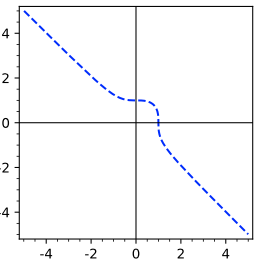
\includegraphics{Midterm2/1.png}
    \caption{$\alpha = 1$}
    \label{fig:my_label}
\end{figure}

\begin{figure}
    \centering
    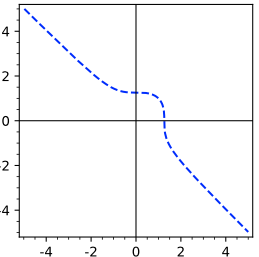
\includegraphics{Midterm2/2.png}
    \caption{$\alpha = 2$}
    \label{fig:my_label}
\end{figure}

\begin{figure}
    \centering
    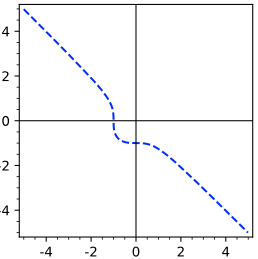
\includegraphics{Midterm2/-1.png}
    \caption{$\alpha = -1$}
    \label{fig:my_label}
\end{figure}
    
\end{document}